
% This LaTeX was auto-generated from MATLAB code.
% To make changes, update the MATLAB code and republish this document.

\documentclass{article}
\usepackage{graphicx}
\usepackage{color}

\sloppy
\definecolor{lightgray}{gray}{0.5}
\setlength{\parindent}{0pt}

\begin{document}

    
    
\subsection*{Contents}

\begin{itemize}
\setlength{\itemsep}{-1ex}
   \item System
   \item Section 1: Translation Controller Design -\ensuremath{>} Marginally Stable Pole at the Origin
   \item Section 2: Translation Controller Design -\ensuremath{>} Unstable Double-Pole at the Origin
   \item Section 3: Translation Controller Design -\ensuremath{>} Unstable Double-Pole at the Origin
   \item Simulation
   \item Coordinate Feedback
\end{itemize}
\begin{verbatim}
% Astrobee Model
\end{verbatim}


\subsection*{System}

\begin{verbatim}
% A Matrix

load Matrices/A_matrix.mat
A = A_matrix

% B Matrix: Stowed

load Matrices/B_stowed.mat
B = B_stowed

% Full-State Feedback

Cf = eye(12);

Df = [zeros(12, 6)];

sys_full = ss(A, B, Cf, Df);

tf_full = tf(sys_full);

syms s

tf_full_sym = simplify(Cf * inv(s * eye(12) - A) * B + Df);
pretty(tf_full_sym)
\end{verbatim}

        \color{lightgray} \begin{verbatim}A =
     0     0     0     0     0     0     0     0     0     0     0     0
     0     0     0     0     0     0     0     0     0     0     0     0
     0     0     0     0     0     0     0     0     0     0     0     0
     0     0     0     0     0     0     0     0     0     0     0     0
     0     0     0     0     0     0     0     0     0     0     0     0
     0     0     0     0     0     0     0     0     0     0     0     0
     1     0     0     0     0     0     0     0     0     0     0     0
     0     1     0     0     0     0     0     0     0     0     0     0
     0     0     1     0     0     0     0     0     0     0     0     0
     0     0     0     1     0     0     0     0     0     0     0     0
     0     0     0     0     1     0     0     0     0     0     0     0
     0     0     0     0     0     1     0     0     0     0     0     0
B =
    0.0630         0         0         0         0         0
         0    0.0630         0         0         0         0
         0         0    0.0630         0         0         0
         0         0         0    5.4054         0         0
         0         0         0         0    4.9505         0
         0         0         0         0         0    5.3191
         0         0         0         0         0         0
         0         0         0         0         0         0
         0         0         0         0         0         0
         0         0         0         0         0         0
         0         0         0         0         0         0
         0         0         0         0         0         0
/   500                                        \
| ------,    0,      0,     0,      0,     0   |
| 7939 s                                       |
|                                              |
|           500                                |
|    0,   ------,    0,     0,      0,     0   |
|         7939 s                               |
|                                              |
|                   500                        |
|    0,      0,   ------,   0,      0,     0   |
|                 7939 s                       |
|                                              |
|                           200                |
|    0,      0,      0,    ----,    0,     0   |
|                          37 s                |
|                                              |
|                                  500         |
|    0,      0,      0,     0,    -----,   0   |
|                                 101 s        |
|                                              |
|                                          250 |
|    0,      0,      0,     0,      0,    ---- |
|                                         47 s |
|                                              |
|   #1,      0,      0,     0,      0,     0   |
|                                              |
|    0,     #1,      0,     0,      0,     0   |
|                                              |
|    0,      0,     #1,     0,      0,     0   |
|                                              |
|                          200                 |
|    0,      0,      0,   -----,    0,     0   |
|                             2                |
|                         37 s                 |
|                                              |
|                                  500         |
|    0,      0,      0,     0,   ------,   0   |
|                                     2        |
|                                101 s         |
|                                              |
|                                         250  |
|    0,      0,      0,     0,      0,   ----- |
|                                            2 |
\                                        47 s  /

where

           500
   #1 == -------
               2
         7939 s


\end{verbatim} \color{black}
    

\subsection*{Section 1: Translation Controller Design -\ensuremath{>} Marginally Stable Pole at the Origin}

\begin{verbatim}
% Top-half matrix (t1):

% Satisfaction of the first interpolation condition

translation_full = [tf_full_sym(1:3, 1:3); tf_full_sym(7:9, 1:3)];
pretty(translation_full);

Gp_t1 = translation_full(1:3, 1:3);
P_t1 = Gp_t1 * s;

[UL_t1, UR_t1, S_t1] = smithForm(P_t1, s)

Mp_t1 = S_t1/s

K_t1 = 1;
tp_t1 = 100;

Y1 = (K_t1 * s)/(tp_t1 * s + 1);
Y2 = Y1;
Y3 = Y1;

My_t1 = diag([Y1 Y2 Y3])

Mt = Mp_t1 * My_t1

Gc_t1_sym = simplify((UR_t1 * inv(eye(size(My_t1 * Mp_t1)) - My_t1 * Mp_t1) * My_t1 * UL_t1))

Gc_t1 = tf(double(Gc_t1_sym));

% % Convert to a string
% Gc_t1_arr = [zeros(1, 3)];
% Gc_t1_str = [];
% for i = 1:size(Gc_t1_sym, 1)
%         Gc_t1_str = char(Gc_t1_sym(i, i));
%         % Define ?s? as transfer function variable
%         s = tf('s');
%         % Evaluate the expression:
%         eval(Gc_t1_arr(i) == Gc_t1_str)
% end
%
% Gc_t1 = diag(Gc_t1_arr)
\end{verbatim}

        \color{lightgray} \begin{verbatim}/    500                    \
|  ------,    0,       0    |
|  7939 s                   |
|                           |
|             500           |
|    0,     ------,    0    |
|           7939 s          |
|                           |
|                      500  |
|    0,       0,     ------ |
|                    7939 s |
|                           |
|   500                     |
| -------,    0,       0    |
|       2                   |
| 7939 s                    |
|                           |
|            500            |
|    0,    -------,    0    |
|                2          |
|          7939 s           |
|                           |
|                     500   |
|    0,       0,    ------- |
|                         2 |
\                   7939 s  /

UL_t1 =
[ 0, 0, 1]
[ 0, 1, 0]
[ 1, 0, 0]
UR_t1 =
[        0,        0, 7939/500]
[        0, 7939/500,        0]
[ 7939/500,        0,        0]
S_t1 =
[ 1, 0, 0]
[ 0, 1, 0]
[ 0, 0, 1]
Mp_t1 =
[ 1/s,   0,   0]
[   0, 1/s,   0]
[   0,   0, 1/s]
My_t1 =
[ s/(100*s + 1),             0,             0]
[             0, s/(100*s + 1),             0]
[             0,             0, s/(100*s + 1)]
Mt =
[ 1/(100*s + 1),             0,             0]
[             0, 1/(100*s + 1),             0]
[             0,             0, 1/(100*s + 1)]
Gc_t1_sym =
[ 7939/50000,          0,          0]
[          0, 7939/50000,          0]
[          0,          0, 7939/50000]
\end{verbatim} \color{black}
    

\subsection*{Section 2: Translation Controller Design -\ensuremath{>} Unstable Double-Pole at the Origin}

\begin{verbatim}
% Bottom-half matrix (t2):

% Run this section first to calculate 'tz' to ensure that the second interpolation condition is satisfied

% d^k(T)/ds^k|(s=0) = 0, where k = 1 (since there is a double unstable pole
% (multiplicity ap = 2) in the plant at s = 0; k = ap - 1) -> 2nd
% interpolation condition

C_t2 = 500/7939; % Constant
Wn = 0.01; % Natural Frequency of the Control System
K = Wn^2/C_t2; % Controller Gain
Z = 2^-0.5; % Damping Ratio
tp = 1/(10*Wn); % Time constant (of the included pole)

syms s tz

TF = ((K*C_t2)*(tz*s + 1))/((s^2 + 2*Z*Wn*s + Wn^2)*(tp*s + 1))
dTF = diff(TF,s)
eqn = subs(dTF,s,0) == 0;
tz = solve(eqn,tz)
\end{verbatim}

        \color{lightgray} \begin{verbatim}TF =
((s*tz)/10000 + 1/10000)/((10*s + 1)*(s^2 + (2^(1/2)*s)/100 + 1/10000))
dTF =
tz/(10000*(10*s + 1)*(s^2 + (2^(1/2)*s)/100 + 1/10000)) - (10*((s*tz)/10000 + 1/10000))/((10*s + 1)^2*(s^2 + (2^(1/2)*s)/100 + 1/10000)) - (((s*tz)/10000 + 1/10000)*(2*s + 2^(1/2)/100))/((10*s + 1)*(s^2 + (2^(1/2)*s)/100 + 1/10000)^2)
tz =
100*2^(1/2) + 10
\end{verbatim} \color{black}
    

\subsection*{Section 3: Translation Controller Design -\ensuremath{>} Unstable Double-Pole at the Origin}

\begin{verbatim}
% Youla Control Design

s = tf('s');

% Constants & Design Parameters
C_t2 = 500/7939; % Constant
Wn = 0.01; % Natural Frequency of the Control System
K = Wn^2/C_t2; % Controller Gain
Z = 2^-0.5; % Damping Ratio
tp = 1/(10*Wn); % Time Constant of the added pole
tz = 100*2^(1/2) + 10;

% Plant TF, 'Gp'
Gp = zpk(minreal(C_t2/s^2))

% Chosen Youla Parameter, 'Y' -> Y(0) = 0
Y = zpk(minreal(((K*s^2)*(tz*s + 1)/((s^2 + 2*Z*Wn*s + Wn^2)*(tp*s + 1))),1e-05))

% Complementary Sensitivity TF, 'T' -> T(0) = 1 (1st interpolation
% condition)
T = zpk(minreal((Y*Gp),1e-05))

% Sensitivity TF, 'S'
S = zpk(minreal((1-T),1e-05))

% Controller TF, 'Gc'
Gc = zpk(minreal((Y/S),1e-05))

% Return Ratio, 'L'
L = zpk(minreal((Gc*Gp),1e-05))

GpS = zpk(minreal((Gp*S),1e-05))

% Internal stability check
Y_stability = isstable(Y)
T_stability = isstable(T)
S_stability = isstable(S)
GpS_stability = isstable(GpS)

M2 = 1/getPeakGain(S) % M2-margin
BW = bandwidth(T) % Bandwidth of the closed-loop
AE = getPeakGain(Y) % Maximum actuator effort

figure(1)
bodemag(Y, S, T);
legend('Y','S','T');

Gc_t2 = [tf(Gc) 0 0; 0 tf(Gc) 0; 0 0 tf(Gc)]

% Convert to symbolic matrix
[Num,Den] = tfdata(tf(Gc), 'v')
syms s
Gc_t2_sym_term = poly2sym(Num, s)/poly2sym(Den, s)
Gc_t2_sym = diag([Gc_t2_sym_term Gc_t2_sym_term Gc_t2_sym_term])

Gc_t = [Gc_t1_sym Gc_t2_sym]
\end{verbatim}

        \color{lightgray} \begin{verbatim}
Gp =
 
  0.06298
  -------
    s^2
 
Continuous-time zero/pole/gain model.


Y =
 
      0.024043 s^2 (s+0.006604)
  ---------------------------------
  (s+0.1) (s^2 + 0.01414s + 0.0001)
 
Continuous-time zero/pole/gain model.


T =
 
       0.0015142 (s+0.006604)
  ---------------------------------
  (s+0.1) (s^2 + 0.01414s + 0.0001)
 
Continuous-time zero/pole/gain model.


S =
 
           s^2 (s+0.1141)
  ---------------------------------
  (s+0.1) (s^2 + 0.01414s + 0.0001)
 
Continuous-time zero/pole/gain model.


Gc =
 
  0.024043 (s+0.006604)
  ---------------------
       (s+0.1141)
 
Continuous-time zero/pole/gain model.


L =
 
  0.0015142 (s+0.006604)
  ----------------------
      s^2 (s+0.1141)
 
Continuous-time zero/pole/gain model.


GpS =
 
         0.06298 (s+0.1141)
  ---------------------------------
  (s+0.1) (s^2 + 0.01414s + 0.0001)
 
Continuous-time zero/pole/gain model.

Y_stability =
  logical
   1
T_stability =
  logical
   1
S_stability =
  logical
   1
GpS_stability =
  logical
   1
M2 =
    0.8909
BW =
    0.0214
AE =
    0.0240

Gc_t2 =
 
  From input 1 to output...
       0.02404 s + 0.0001588
   1:  ---------------------
            s + 0.1141
 
   2:  0
 
   3:  0
 
  From input 2 to output...
   1:  0
 
       0.02404 s + 0.0001588
   2:  ---------------------
            s + 0.1141
 
   3:  0
 
  From input 3 to output...
   1:  0
 
   2:  0
 
       0.02404 s + 0.0001588
   3:  ---------------------
            s + 0.1141
 
Continuous-time transfer function.

Num =
    0.0240    0.0002
Den =
    1.0000    0.1141
Gc_t2_sym_term =
((3464915774230499*s)/144115188075855872 + 5857948048047205/36893488147419103232)/(s + 4112403835698463/36028797018963968)
Gc_t2_sym =
[ ((3464915774230499*s)/144115188075855872 + 5857948048047205/36893488147419103232)/(s + 4112403835698463/36028797018963968),                                                                                                                          0,                                                                                                                          0]
[                                                                                                                          0, ((3464915774230499*s)/144115188075855872 + 5857948048047205/36893488147419103232)/(s + 4112403835698463/36028797018963968),                                                                                                                          0]
[                                                                                                                          0,                                                                                                                          0, ((3464915774230499*s)/144115188075855872 + 5857948048047205/36893488147419103232)/(s + 4112403835698463/36028797018963968)]
Gc_t =
[ 7939/50000,          0,          0, ((3464915774230499*s)/144115188075855872 + 5857948048047205/36893488147419103232)/(s + 4112403835698463/36028797018963968),                                                                                                                          0,                                                                                                                          0]
[          0, 7939/50000,          0,                                                                                                                          0, ((3464915774230499*s)/144115188075855872 + 5857948048047205/36893488147419103232)/(s + 4112403835698463/36028797018963968),                                                                                                                          0]
[          0,          0, 7939/50000,                                                                                                                          0,                                                                                                                          0, ((3464915774230499*s)/144115188075855872 + 5857948048047205/36893488147419103232)/(s + 4112403835698463/36028797018963968)]
\end{verbatim} \color{black}
    
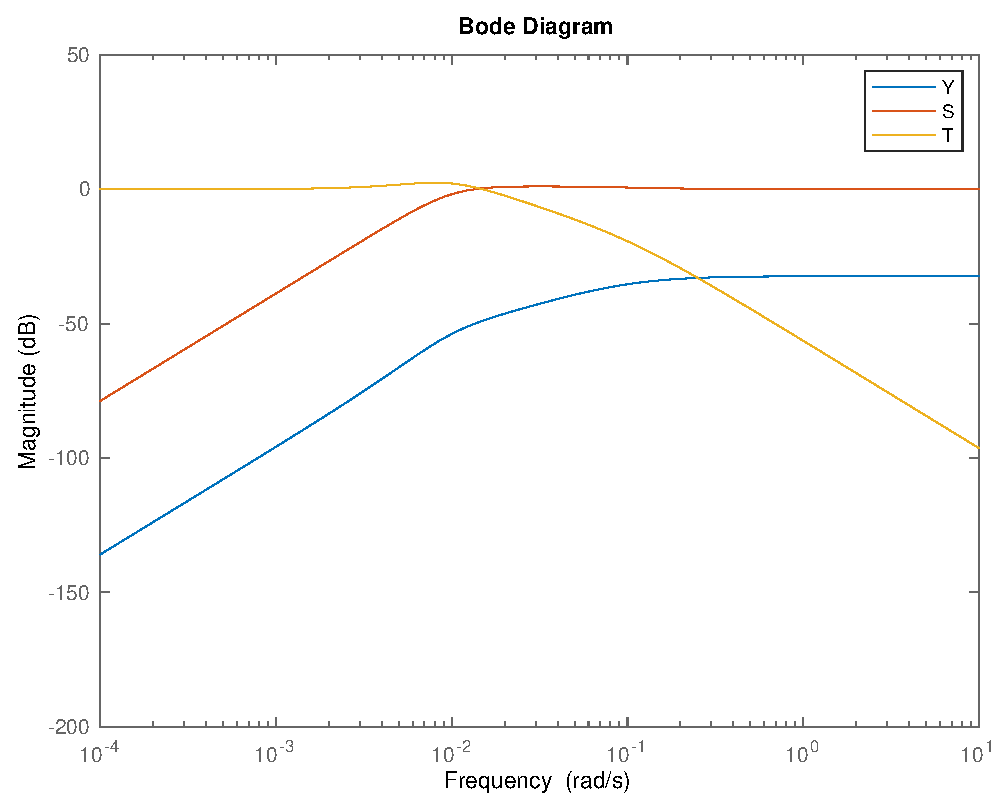
\includegraphics [width=4in]{Astrobee_Euler_Stowed_Translation_01.eps}


\subsection*{Simulation}

\begin{verbatim}
Gp = minreal([tf_full(1:3, 1:3); tf_full(7:9, 1:3)], 1e-05);
Gc = [Gc_t1 Gc_t2]
Lu = minreal(Gc * Gp, 1e-05);
Ly = minreal(Gp * Gc, 1e-05);
Y = minreal(inv(eye(3) + Lu) * Gc);
Ty = minreal(inv(eye(6) + Ly) * Ly);
Sy = minreal(inv(eye(6) + Ly), 1e-05);
Su = minreal(inv(eye(3) + Lu), 1e-05);

figure
step(Ty);

figure
step(Y);

figure
sigma(Y, Ty, Sy, Su)
[l, hObj] = legend('$Y$', '$T_{y}$', '$S_{y}$', '$S_{u}$','Interpreter','latex','FontSize', 12);
set(l,'string',{'$Y$', '$T_{y}$', '$S_{y}$', '$S_{u}$'});
hL = findobj(hObj,'type','line');
set(hL,'linewidth', 2);

figure
sigma(Gc, Gp, Ly, Y)
[l, hObj] = legend('$G_{c}$', '$G_{p}$', '$L_{y}$', '$Y$','Interpreter','latex','FontSize', 12);
set(l,'string',{'$G_{c}$', '$G_{p}$', '$L_{y}$', '$Y$'});
hL = findobj(hObj,'type','line');
set(hL,'linewidth', 2);

figure
sigma(Gc, Gp, Y)
[l, hObj] = legend('$G_{c}$', '$G_{p}$', '$Y$','Interpreter','latex','FontSize', 12);
set(l,'string',{'$G_{c}$', '$G_{p}$', '$Y$'});
hL = findobj(hObj,'type','line');
set(hL,'linewidth', 2);

figure
sigma(Ly, Sy, Ty)
[l, hObj] = legend('$L_{y}$', '$S_{y}$', '$T_{y}$','Interpreter','latex','FontSize', 12);
set(l,'string',{'$L_{y}$', '$S_{y}$', '$T_{y}$'});
hL = findobj(hObj,'type','line');
set(hL,'linewidth', 2);

figure
sigma(Sy, Su)
[l, hObj] = legend('$S_{y}$', '$S_{u}$','Interpreter','latex','FontSize', 12);
set(l,'string',{'$S_{y}$', '$S_{u}$'});
hL = findobj(hObj,'type','line');
set(hL,'linewidth', 2);
\end{verbatim}

        \color{lightgray} \begin{verbatim}
Gc =
 
  From input 1 to output...
   1:  0.1588
 
   2:  0
 
   3:  0
 
  From input 2 to output...
   1:  0
 
   2:  0.1588
 
   3:  0
 
  From input 3 to output...
   1:  0
 
   2:  0
 
   3:  0.1588
 
  From input 4 to output...
       0.02404 s + 0.0001588
   1:  ---------------------
            s + 0.1141
 
   2:  0
 
   3:  0
 
  From input 5 to output...
   1:  0
 
       0.02404 s + 0.0001588
   2:  ---------------------
            s + 0.1141
 
   3:  0
 
  From input 6 to output...
   1:  0
 
   2:  0
 
       0.02404 s + 0.0001588
   3:  ---------------------
            s + 0.1141
 
Continuous-time transfer function.

\end{verbatim} \color{black}
    
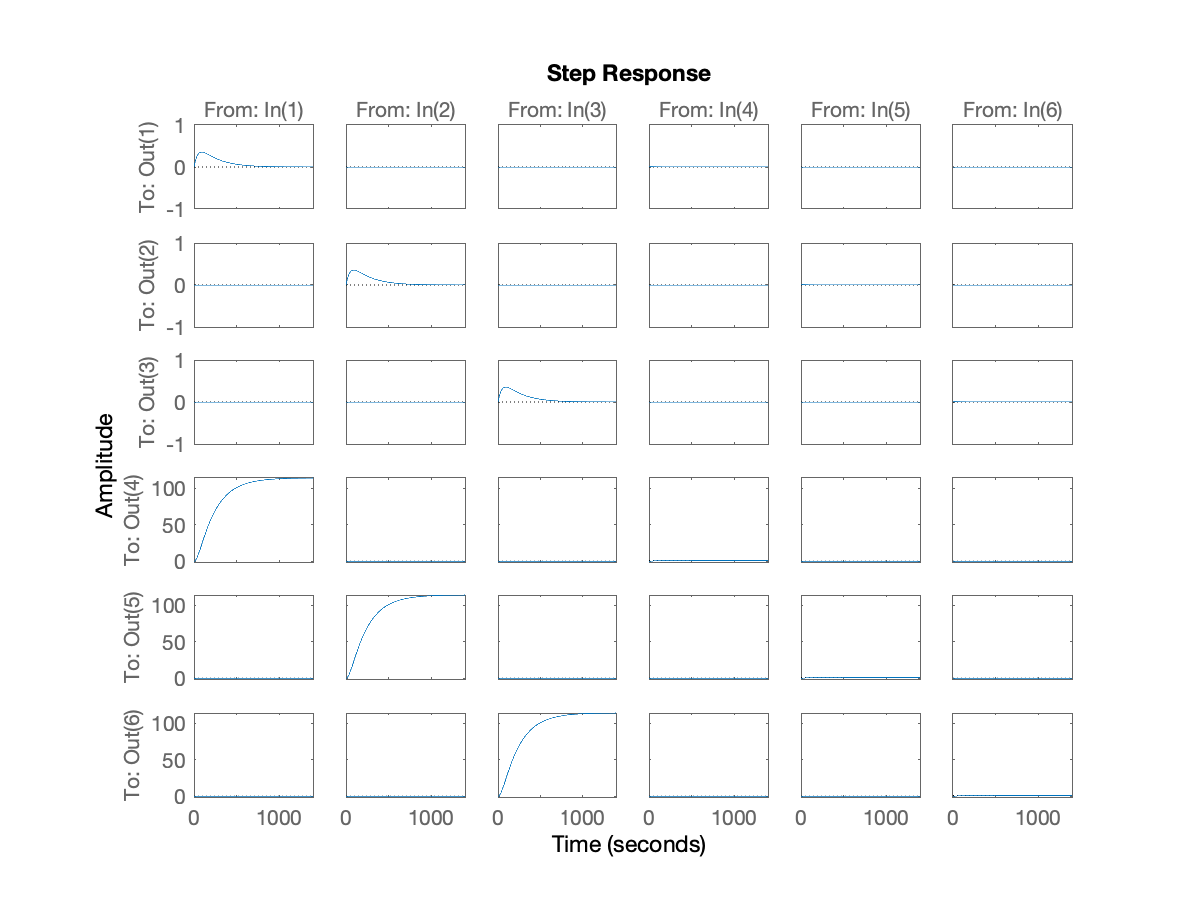
\includegraphics [width=4in]{Astrobee_Euler_Stowed_Translation_02.eps}

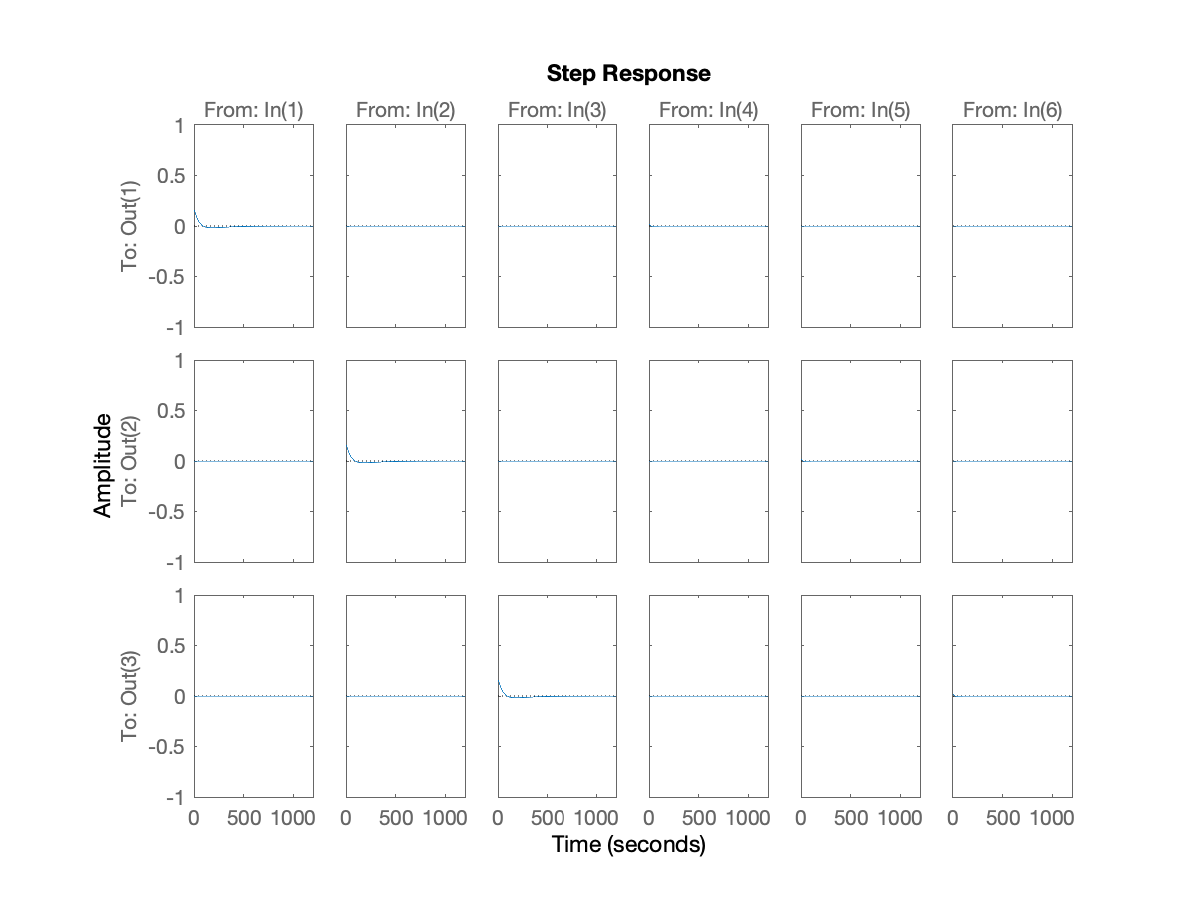
\includegraphics [width=4in]{Astrobee_Euler_Stowed_Translation_03.eps}

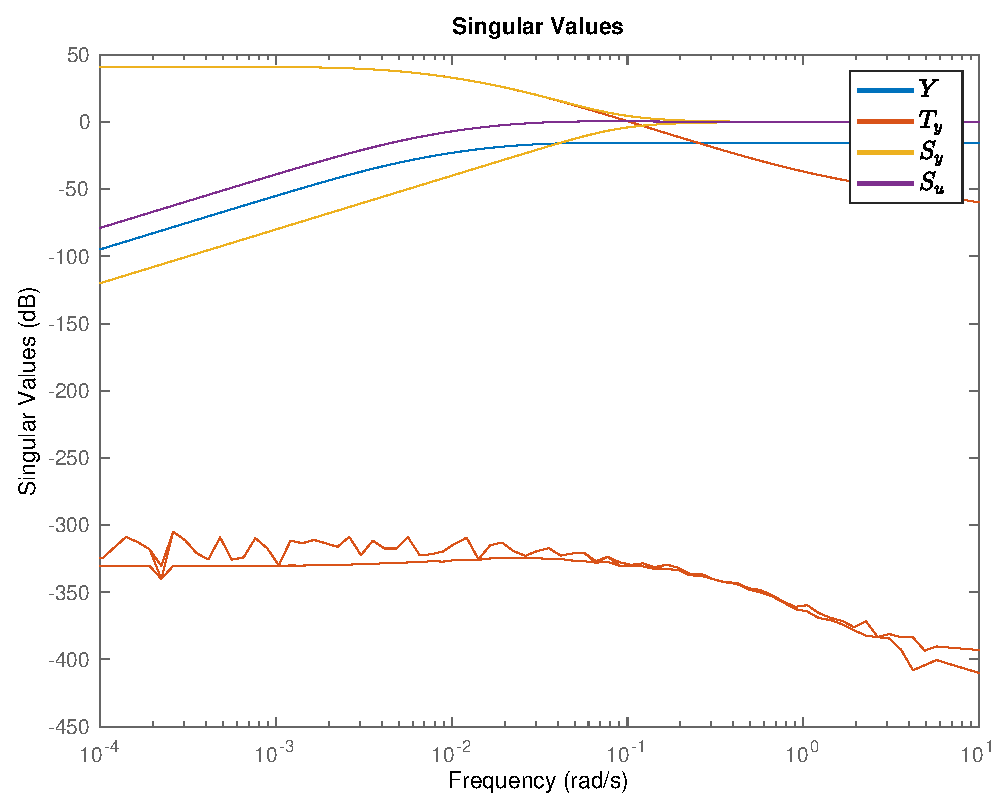
\includegraphics [width=4in]{Astrobee_Euler_Stowed_Translation_04.eps}

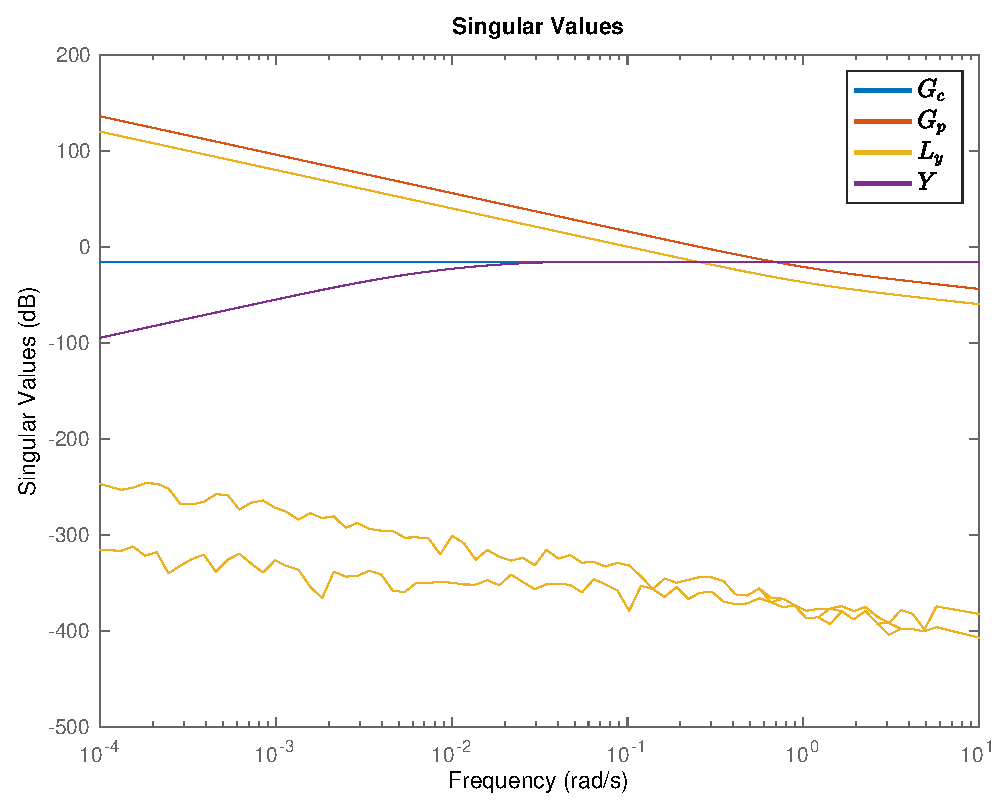
\includegraphics [width=4in]{Astrobee_Euler_Stowed_Translation_05.eps}

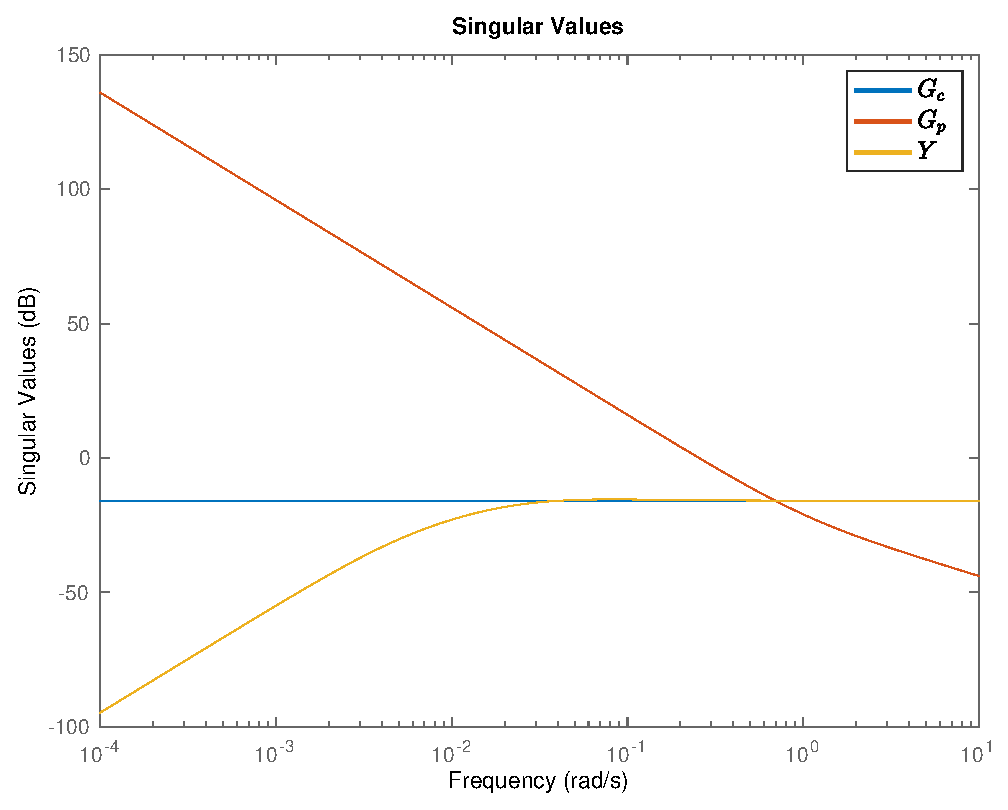
\includegraphics [width=4in]{Astrobee_Euler_Stowed_Translation_06.eps}

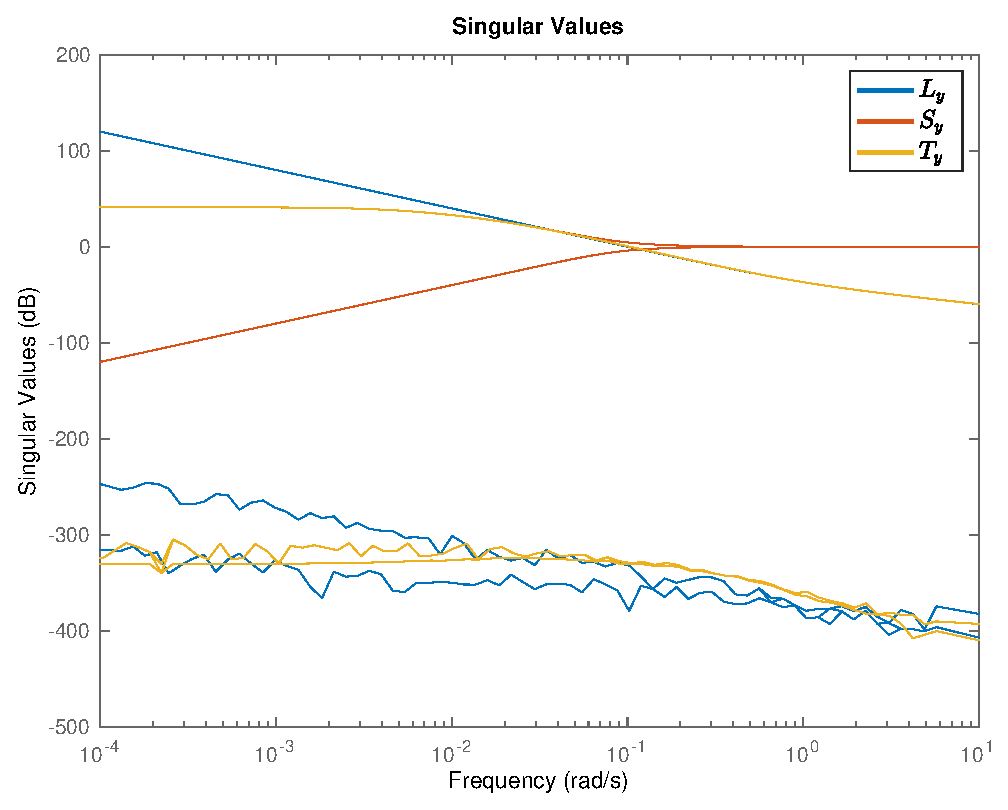
\includegraphics [width=4in]{Astrobee_Euler_Stowed_Translation_07.eps}

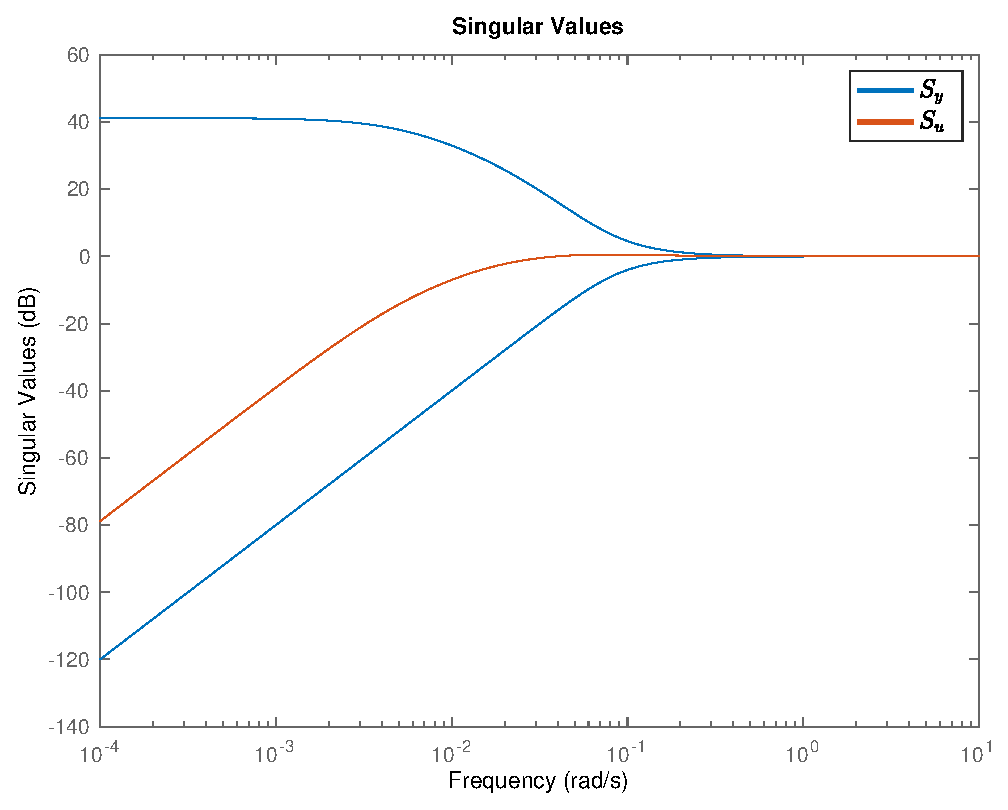
\includegraphics [width=4in]{Astrobee_Euler_Stowed_Translation_08.eps}


\subsection*{Coordinate Feedback}

\begin{verbatim}
% Cc = [zeros(6, 12)];
% Cc(1:6, 1:6) = eye(6);
%
% Dc = [zeros(6, 6)];
%
% sys_coord = ss(A, B, Cc, Dc);
%
% tf_coord = tf(sys_coord);
%
% syms s
%
% tf_coord_sym = simplify(Cc * inv(s * eye(12) - A) * B + Dc);
% pretty(tf_coord_sym)
%
% translation_coord = [tf_coord_sym(1:3, 1:3); tf_coord_sym(7:9, 1:3)];
% pretty(translation_coord)
%
% attitude_coord = [tf_coord_sym(4:6, 4:6); tf_coord_sym(10:12, 4:6)];
% pretty(attitude_coord)
\end{verbatim}



\end{document}
    
